\begin{table}[H]
\centering
\definecolor{tabglobalcrossa0}{rgb}{0.9961,0.7634,0.3684}
\definecolor{tabglobalcrossa1}{rgb}{0.9961,0.7202,0.3219}
\definecolor{tabglobalcrossa2}{rgb}{0.9888,0.3398,0.1744}
\definecolor{tabglobalcrossa3}{rgb}{0.9941,0.6235,0.2658}
\definecolor{tabglobalcrossa4}{rgb}{0.99,0.4173,0.1965}
\definecolor{tabglobalcrossa5}{rgb}{0.8493,0.074,0.1206}
\definecolor{tabglobalcrossa6}{rgb}{0.9915,0.5103,0.2231}
\definecolor{tabglobalcrossa7}{rgb}{0.8072,0.0452,0.1316}
\definecolor{tabglobalcrossa8}{rgb}{0.8773,0.0932,0.1132}
\definecolor{tabglobalcrossa9}{rgb}{0.9094,0.1419,0.1206}
\definecolor{tabglobalcrossa10}{rgb}{0.8306,0.0612,0.1255}
\definecolor{tabglobalcrossa11}{rgb}{0.5845,0.0,0.149}
\definecolor{tabglobalcrossa12}{rgb}{0.9894,0.3785,0.1855}
\definecolor{tabglobalcrossa13}{rgb}{0.7651,0.0164,0.1427}
\definecolor{tabglobalcrossa14}{rgb}{0.502,0.0,0.149}
\definecolor{tabglobalcrossa15}{rgb}{0.891,0.1036,0.1102}
\definecolor{tabglobalcrossa16}{rgb}{0.6971,0.0,0.149}
\definecolor{tabglobalcrossa17}{rgb}{0.8586,0.0804,0.1181}
\definecolor{tabglobalcrossa18}{rgb}{0.8727,0.09,0.1144}
\definecolor{tabglobalcrossa19}{rgb}{0.7838,0.0292,0.1378}
\definecolor{tabglobalcrossa20}{rgb}{1.0,0.9801,0.7513}
\definecolor{tabglobalcrossa21}{rgb}{1.0,0.9402,0.6538}
\definecolor{tabglobalcrossa22}{rgb}{0.9984,0.8971,0.5596}
\definecolor{tabglobalcrossa23}{rgb}{0.9961,0.8498,0.4615}
\definecolor{tabglobalcrossa24}{rgb}{0.9955,0.6781,0.2894}
\definecolor{tabglobalcrossa25}{rgb}{0.9933,0.5962,0.254}
\definecolor{tabglobalcrossa26}{rgb}{0.991,0.4793,0.2143}
\definecolor{tabglobalcrossa27}{rgb}{0.9463,0.2187,0.1412}
\definecolor{tabglobalcrossa28}{rgb}{0.8867,0.0996,0.1107}
\definecolor{tabglobalcrossa29}{rgb}{0.8025,0.042,0.1329}
\definecolor{tabglobalcrossa30}{rgb}{0.7046,0.0,0.149}
\definecolor{tabglobalcrossa31}{rgb}{0.5695,0.0,0.149}
\begin{minipage}{0.78\textwidth}
\centering
\renewcommand{\arraystretch}{1.2}
\begin{tabular}{lccc}
\toprule
Checkpoint & First & Middle & Last \\
\midrule
0 & \cellcolor{tabglobalcrossa0}\textcolor{black}{$0.086 \pm 0.029$} & \cellcolor{tabglobalcrossa1}\textcolor{black}{$0.096 \pm 0.014$} & \cellcolor{tabglobalcrossa2}\textcolor{white}{$0.162 \pm 0.037$} \\
1 & \cellcolor{tabglobalcrossa3}\textcolor{black}{$0.118 \pm 0.025$} & \cellcolor{tabglobalcrossa4}\textcolor{black}{$0.152 \pm 0.028$} & \cellcolor{tabglobalcrossa5}\textcolor{white}{$0.209 \pm 0.052$} \\
5 & \cellcolor{tabglobalcrossa6}\textcolor{black}{$0.139 \pm 0.027$} & \cellcolor{tabglobalcrossa7}\textcolor{white}{$0.219 \pm 0.060$} & \cellcolor{tabglobalcrossa8}\textcolor{white}{$0.203 \pm 0.050$} \\
15 & \cellcolor{tabglobalcrossa9}\textcolor{white}{$0.195 \pm 0.027$} & \cellcolor{tabglobalcrossa10}\textcolor{white}{$0.214 \pm 0.030$} & \cellcolor{tabglobalcrossa11}\textcolor{white}{$0.255 \pm 0.038$} \\
50 & \cellcolor{tabglobalcrossa12}\textcolor{black}{$0.158 \pm 0.023$} & \cellcolor{tabglobalcrossa13}\textcolor{white}{$0.228 \pm 0.046$} & \cellcolor{tabglobalcrossa14}\textcolor{white}{$0.268 \pm 0.047$} \\
200 & \cellcolor{tabglobalcrossa15}\textcolor{white}{$0.200 \pm 0.028$} & \cellcolor{tabglobalcrossa16}\textcolor{white}{$0.240 \pm 0.038$} & \cellcolor{tabglobalcrossa17}\textcolor{white}{$0.208 \pm 0.035$} \\
last & \cellcolor{tabglobalcrossa18}\textcolor{white}{$0.204 \pm 0.028$} & \cellcolor{tabglobalcrossa16}\textcolor{white}{$0.240 \pm 0.038$} & \cellcolor{tabglobalcrossa19}\textcolor{white}{$0.224 \pm 0.043$} \\
\bottomrule
\end{tabular}
\end{minipage}%
\hfill
\begin{minipage}{0.15\textwidth}
\centering
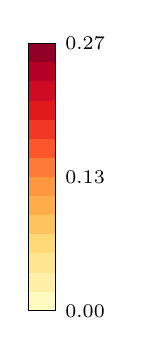
\begin{tikzpicture}
\fill[tabglobalcrossa20] (0,0.0000) rectangle (0.35,0.2429);
\fill[tabglobalcrossa21] (0,0.2429) rectangle (0.35,0.4857);
\fill[tabglobalcrossa22] (0,0.4857) rectangle (0.35,0.7286);
\fill[tabglobalcrossa23] (0,0.7286) rectangle (0.35,0.9714);
\fill[tabglobalcrossa0] (0,0.9714) rectangle (0.35,1.2143);
\fill[tabglobalcrossa24] (0,1.2143) rectangle (0.35,1.4571);
\fill[tabglobalcrossa25] (0,1.4571) rectangle (0.35,1.7000);
\fill[tabglobalcrossa26] (0,1.7000) rectangle (0.35,1.9429);
\fill[tabglobalcrossa2] (0,1.9429) rectangle (0.35,2.1857);
\fill[tabglobalcrossa27] (0,2.1857) rectangle (0.35,2.4286);
\fill[tabglobalcrossa28] (0,2.4286) rectangle (0.35,2.6714);
\fill[tabglobalcrossa29] (0,2.6714) rectangle (0.35,2.9143);
\fill[tabglobalcrossa30] (0,2.9143) rectangle (0.35,3.1571);
\fill[tabglobalcrossa31] (0,3.1571) rectangle (0.35,3.4000);
\draw[black,line width=0.3pt] (0,0) rectangle (0.35,3.4000);
\node[right,font=\scriptsize,anchor=west] at (0.35,3.4000) {0.27};
\node[right,font=\scriptsize,anchor=west] at (0.35,1.7000) {0.13};
\node[right,font=\scriptsize,anchor=west] at (0.35,0) {0.00};
\end{tikzpicture}
\end{minipage}
\caption{Global cross-comparison, Direction A (both normalised, different training objective). Mean $\pm$ SE across 10 datasets (First/Last), 8 for Middle (datasets with $L=2$ contribute no middle layer). (Pooled fold/layer SE averages 0.011 across cells; not shown per cell, see text.) Cell shading: white = 0, dark red = 0.27 (max value in this table), YlOrRd colormap, same scale as Fig.~\ref{fig: RM_Norm} etc.}
\label{tab:global_cross_a}
\end{table}
